% "Plain" Template for PHENIX Physics Paper submission to PRL or PRC or PRD
%
% The /phenix/WWW/p/info/dp/000/template/template4.tex file has embedded hints.
%
%      [Modified by Brant to uncomment line numbers on Feb. 15, 2009]
%      [Modified by Brant to change to revtex4-1 and longbibliography,
%               to include titles in reference lists, June, 2015]
%      [Modified by Brant to remove "showpacs" on April 9, 2018]

% Please see help files in  /phenix/WWW/p/info/dp/000/template/
% and then ask Brant <brant@bnl.gov>, if you have any questions about the
% preparation of your draft.
%
%   Copyright (c) 2001 The American Physical Society.
%
% This is a template for producing manuscripts for use with REVTEX 4.0
% Copy this file to another name and then work on that file.

%%%%%%%%%%%%%%%%%%%   **** NEW PHENIX custom *****  %%%%%%%%%%%%%%%%%%%%
% Use linenumbers for PPG drafting and internal releases.  Brant
% will commment out these lines before submission to arXiv and journal.
\RequirePackage{lineno}
\setlength{\linenumbersep}{6pt}
\linenumbers
% [NOTE: you also need access to this file:
% /phenix/WWW/p/info/dp/000/template/lineno.sty

%%%%%%%%%%%%%%%%%%% figures in subdirectories  %%%%%%%%%%%%%%%%%%%%%%%
%% The arXiv and journals require a flat file structure with all
%% figure files in the same directory as the single .tex file
%% However, some authors (especially for long PRC or PRD) find it useful
%% to use subdirectories for the figures either below the working
%% directory (./fig1/) or at the same directory level (../fig2/).
%% If so, then edit and uncomment:
%\graphicspath{{./}{./figs1/}{../figs2/}}

% Before starting the draft, please carefully review the template files:
%    https://www.phenix.bnl.gov/phenix/WWW/p/info/dp/000/template
% This is Template4_plain.tex (without all the embedded hints).
% You may also choose to use Template4.tex (with all the embedded hints).

% Please select the "twocolumn" option below for your intended journal.
% Brant will later select the "onecolumn" option for APS journal submission 
% format or will transform everything to be appropriate for PLB, NPA, etc. 

% For Phys. Rev. Lett. choose (uncomment) one of:
\documentclass[twocolumn,letterpaper,aps,prl,longbibliography,superscriptaddress,floatfix]{revtex4-2}
%\documentclass[onecolumn,letterpaper,aps,prl,longbibliography,superscriptaddress,floatfix]{revtex4-1}

% For Phys. Rev. C choose (uncomment) one of:
%\documentclass[twocolumn,letterpaper,aps,prc,longbibliography,superscriptaddress,nofootinbib,floatfix]{revtex4-1}
%\documentclass[onecolumn,letterpaper,aps,prc,longbibliography,superscriptaddress,nofootinbib,floatfix]{revtex4-1}

% For Phys. Rev. D choose (uncomment) one of:
%\documentclass[twocolumn,letterpaper,aps,prd,longbibliography,superscriptaddress,nofootinbib,floatfix]{revtex4-1}
%\documentclass[onecolumn,letterpaper,aps,prd,longbibliography,superscriptaddress,nofootinbib,floatfix]{revtex4-1}

\usepackage{amsmath}
\usepackage{amsfonts}
\usepackage{amssymb}
\usepackage{slashed}
\usepackage{graphicx}
\usepackage{tikz-feynman}
\usepackage{float}

\newcommand{\pT}{\ensuremath{p_T}}
\newcommand{\pizero}{\ensuremath{\pi^0}}
\newcommand{\ALL}{\ensuremath{A_{LL}}}

\begin{document}

%%%%%%%%%%%%%%%%%%%%%%%%%%%%%%%%%%%%%%%%%%%%%%%%% Title of paper

%%%%% NOTE:  Use the above macros in text and captions, but not in 
%%%%%        the title or abstract.  Those two elements must stand
%%%%%        alone and not be dependent on the macros defined here.

\title{Measurement of Direct Photon Cross Section and Double Helicity Asymmetry at $\sqrt{s}$ = 510 GeV in $\vec{p}+\vec{p}$ Collisions at PHENIX}

\author{PHENIX Collaboration Author List (Brant will insert later)}

\date{\today}

\begin{abstract}
Understanding the gluon spin contribution to the proton spin is among the primary motivations of the spin program at the Relativistic Heavy Ion Collider (RHIC) \cite{aschenauer2015rhic}. Double helicity asymmetry $A_{LL}$ of direct photon production in $\vec{p}+\vec{p}$ collisions at RHIC is sensitive to the gluon helicity in the polarized proton. Direct photons are dominantly produced by the quark-gluon Compton process at RHIC energies, and utilizing an isolation criteria can reduce the fragmentation contributions and photons from hadronic decays. The asymmetry measurement with isolation criteria provides clean access to the polarization of the gluon. We present the cross section and double helicity asymmetry measurements of direct photon production in longitudinally polarized proton collisions at $\sqrt{s}$ = 510 GeV at midrapidity ($|\eta| <$ 0.25). These data are expected to provide additional constraints on the gluon helicity distribution in the gluon momentum fraction range 0.02 $< x <$ 0.08.
\end{abstract}

% insert suggested PACS numbers in braces on next line
\pacs{14.20.Dh, 13.60.Hb, 21.10.Hw, 24.85.+p}
	
%\maketitle must follow title, authors, abstract, \pacs, and \keywords
\maketitle

%\section{Justification of PRL}

%Understanding how much proton spin comes from gluon helicity is important to solve the proton spin puzzle. Though there are many ways to probe the gluon heliciy, e.g. through gluon fusion in polarized deep inelastic scattering or hadrons/jets production in polarized $\vec{p}+\vec{p}$ collions, they are either at next-to-leading order or suffering from large systematic uncertainty of fragmentation processes. On the other hand, the direct photon production in $\vec{p}+\vec{p}$ gives a clean probe to the gluon helicity at leading order with little fragmentation contributions. This ``gloden'' channel was limited by statistics until the RHIC run of year 2013, which provides the largest statistics for $\vec{p}+\vec{p}$ collisions at the only existing polarized proton collider. The measured double helicity asymmetries \ALL\ will play an essential role in the future global fitting to extract the gluon helicity inside the proton at Bjorken x from 0.02 to 0.08. This will be the first direct photon cross section measurement at $\sqrt{s}$ = 510 GeV and the first direct photon \ALL\ measurement.

%%% To check PRL length insert this (uncommented) line after \\maketitle:
\textbf{*** page break for PRL word count ***}  \clearpage
%%% and see below.

%Direct photons are produced in a collision before the formation of hadrons. Due to this reason, as well as they can penetrate the medium formed in the collision, it is an excellent probe to the initial state of the hadrons or heavy ions. At leading order, there are four processes that contribute to direct photon production in proton-proton collisions: quark-gluon Compton scattering, quark-antiquark annihilation, parton fragmentation, and quark bremsstrahlung. Among them, most direct photons are produced by $qg \rightarrow q\gamma$ scattering. As a result, it is a clean probe of the gluon distribution inside the proton and provides an independent test of perturbative Quantum Chromodynamics (pQCD). It also provides a baseline for direct photon production in heavy ion collisions.

Direct photons, which are photons not from hadronic decays, are produced in hadron-hadron collisions by charged particles such as quarks. Unlike hadrons and jets, direct photons do not participate in strong interactions at leading-order perturbative Quantum Chromodynamics (pQCD) and provide a clean probe to the initial state of hadrons. The majority of direct photons with transverse momentum larger than 5 GeV/c are produced by quark-gluon Compton scattering $qg \rightarrow q\gamma$ in proton-proton collisions at Relativistic Heavy Ion Collider (RHIC) energies. This process is linear in gluon parton distribution function (PDF) and with little final-state fragmentation contributions involved. Due to this reason, direct photon production is the ``golden'' channel to probe the (un)polarized gluon PDF inside the proton and is proposed by RHIC spin plan decades ago \cite{aschenauer2015rhic}. Other contributions to the direct photon production at leading-order pQCD include quark-antiquark annihilation, quark fragmentation and bremstraulung.

In polarized proton collisions, spin asymmetry measurements are sensitive to the polarized structure of the proton and allow one to investigate its spin decomposition. Determining how fundamental properties of a particle such as spin are composed of its constituents is of great importance in understanding the theory that describes nature. pQCD has been successful in describing unpolarized cross sections while spin-dependent observables have historically offered more of a challenge. Measurements of such quantities enable us to study the theory in greater depth. Polarized deep-inelastic scattering (DIS) has shown that only part of the proton spin is carried by quark spins, and a large fraction of it appears to be carried by gluons and orbital angular momentum \cite{1988364, ALEXAKHIN20078}. In DIS measurements gluons are usually involved at higher orders and the polarized gluon distribution has been left nearly unconstrained due to the limited data and kinematic coverage. At RHIC, various scattering processes involve gluons at leading-order making them more readily accessible. Measurement of double helicity asymmetry of such processes in longitudinally polarized $p+p$ collisions are directly sensitive to the polarized gluon distribution. Recent RHIC measurements of \pizero and jets \cite{PhysRevD.90.012007, PhysRevLett.103.012003, PhysRevD.79.012003, PhysRevD.86.032006, PhysRevLett.115.092002} included in global analyses have shown the first direct evidence of nonzero gluon spin contributions to the spin of the proton \cite{PhysRevLett.113.012001} in the Bjorken-x range larger than 0.05. Measurements at higher energy $\sqrt{s}$ = 510 GeV \cite{PhysRevD.93.011501, PhysRevD.100.052005} have confirmed the nonzero gluon polarization and extended the minimum x reach to $\sim$0.01. Unlike hadrons, direct photon production does not involve final-state effects leading to a more straightforward theoretical interpretation. Moreover, it can provide a complementary constraint on the polarized gluon distribution.

In this Letter, we present the first measurements of inclusive and isolated direct photon cross sections and double helicity asymmetry \ALL\ of isolated photons at $\sqrt{s}$ = 510 GeV at $|\eta| <$ 0.25 from the 2013 RHIC run. The data were collected with the PHENIX detector \cite{ADCOX2003469}. The primary detector for this measurement is an electromagnetic calorimeter (EMCal) \cite{APHECETCHE2003521}, consisting of two subsystems, a six sector lead-scintillator (PbSc), and a two sector lead glass (PbGl) detector, each located 5 m radially from the beam line. Each sector covers a range of  $|\eta| <$ 0.35 in pseudorapidity and 22.5\textdegree\ in azimuth. The EMCal has fine granularity with each tower covering $\Delta\eta \times \Delta\phi \sim$ 0.01 $\times$ 0.01 (0.008 $\times$ 0.008) for PbSc (PbGl). Two photons from $\pi^0 \rightarrow \gamma\gamma$ decays are clearly resolved up to a \pizero\ \pT\ of 12 GeV/c, and a shower profile analysis extends the $\gamma/\pi^0$ discrimination to beyond 20 GeV/c. The energy calibration of each tower is obtained from the reconstructed \pizero\ mass.

%The MB trigger cross section is $\sigma_{BBC}$ = 32.51 $\pm$ 3.01(syst) $\pm$ 1.19(stat) mb. The efficiency bias due to the MB trigger in the 2013 run, $\epsilon_{BBC}$ = 0.91 $\pm$ 0.01, is determined from the ratio of the yield of high \pT\ \pizero\ with and without the MB trigger. 

%% photon clustering, event cuts here
%The first step in the analysis is to cluster the hit towers. If there are two tower energy maxima and at least one lower energy tower between them, the cluster is split into two, with the energy of each tower divided between the two clusters according to electromagnetic shower profiles associated with the clusters.

The Beam-Beam Counters (BBC) \cite{ALLEN2003549} cover 3.1 $< |\eta| <$ 3.9 and are located at $\pm$ 144 cm from the interaction point along the beam line. The BBCs measure the collision vertex and provide a minimum-bias (MB) trigger. The BBCs are also used as a luminosity monitor. Events with high \pT\ photons are selected by a EMCal-based trigger requiring a minimum energy deposit of 3.7 GeV in an overlapping tile of 4 $\times$ 4 towers of the EMCal in coincidence with the MB trigger. An integrated luminosity ($\mathcal{L}$) of 33 (108) pb$^{-1}$ with a z-vertex requirement of 10 (30) cm around the nominal interaction point is used in the cross section (\ALL) analysis.
 
The photon reconstruction and analysis method used here is similar to the previous PHENIX measurement at $\sqrt{s}$ =  200 GeV \cite{PhysRevLett.98.012002,PhysRevD.86.072008}. Photons are identified by a shower profile requirement that was calibrated using test beam data, identified electrons, and decay photons from identified \pizero. This requirement rejects $\sim$50\% of hadrons depositing E $>$ 3 GeV in the EMCal and accepts $\sim$98\% of real photons. A time-of-flight requirement $|ToF| <$ 10 ns is used to reduce pile-up events due to high collision rate and a minimum energy requirement $E_{min} >$ 0.3 GeV is applied to reduce the background noise in the EMCal. The charged particle veto of the photon sample is based on tracks in drift chambers (DC) \cite{ADCOX2003489}. 

The experimental challenge in this measurement is the large photon background from hadron decays, primarily from $\pi^0 \rightarrow \gamma\gamma$ ($\sim$80\% of the decays) and $\eta \rightarrow \gamma\gamma$ ($\sim$15\%). Photon candidates that form a pair with another photon in the mass range 110 $< M_{\gamma\gamma} <$ 160 MeV ($M_{\pi^0} \pm 3\sigma$) with $E_{\gamma} >$ 300 MeV are tagged as \pizero\ decay photons. A fiducial region for direct photon candidates excludes 10 towers (0.1 rad) from the edges of the EMCal while partner photons are accepted over the entire detector to improve the probability of observing both decay photons from the \pizero. This method overestimates $\sim$8\% more yield of photons from \pizero\ decays, $\gamma_{\pi^0}^{inc}$, due to combinatorial background. A \pT\ dependent correction is estimated from the fit of the background under \pizero\ peak in two-photon invariant mass distribution. The inclusive direct photon yield is then written as

\begin{equation} \label{eq:inc}
\gamma_{dir}^{inc} = \gamma_{total}^{inc} - \left( 1 + R_{\pi^0}^{miss} + \delta_{h/\pi^0}^{\gamma} \right) \gamma_{\pi^0}^{inc},
\end{equation}
where we subtract the reconstructed inclusive \pizero's decay photons ($\gamma_{\pi^0}^{inc}$), those missing their partner photons ($R_{\pi^0}^{miss}\gamma_{\pi^0}^{inc}$) and photons from other hadron decays ($\delta_{h/\pi^0}^{\gamma}\gamma_{\pi^0}^{inc}$) from total inclusive photons ($\gamma_{total}^{inc}$). If a partner photon of a \pizero\ decay is missed, it will not be reconstructed in the \pizero\ mass peak window. The ratio of photons with missing partner photons over decay photons from reconstructed \pizero\, $R_{\pi^0}^{miss}$, is estimated using a simulation.
$\delta_{h/\pi^0}^{\gamma}$ is calculated by $\eta$, $\omega$, $\eta'$ over \pizero\ ratios based on the previous 200 GeV measurement\cite{PhysRevD.83.052004}: $\delta_{h/\pi^0}^{\gamma} \approx$ 0.28, with $\delta_{\eta/\pi^0}^{\gamma} \approx$ 0.21 and $\delta_{\omega/\pi^0}^{\gamma} \approx \delta_{\eta'/\pi^0}^{\gamma}  \approx$ 0.035. A PYTHIA \cite{Sjostrand:2006za} simulation showed that the variation of these ratios is less than 10\% between 200 GeV and 510 GeV in 6 $< p_T <$ 30 GeV/c. The difference is accounted for by assigning a systematic uncertainty.

In addition, an isolation requirement is also applied, which can largely reduce the contributions from parton fragmentation and hadron decays. For any other particles within a cone of radius $r_{cone} = \sqrt{(\delta\eta)^2 + (\delta\phi)^2} = 0.5$ of the signal photon, the sum of their energies is required to be less than 10\% of the energy of the signal photon: $E_{cone} < 0.1 E_{\gamma}$. Similar to Eq. (\ref{eq:inc}), the isolated direct photon yield can be expressed as

%We measure the energy of charged particles by their momenta in DC and that of neutral particles by EMCal: $\sum E_{neutral} + \sum E_{charged} < 0.1E_{\gamma}$. The resultant isolated direct photon yield is

\begin{equation} \label{eq:iso}
\gamma_{dir}^{iso} = \gamma_{total}^{iso} - \gamma_{\pi^0}^{iso} - \left( R_{\pi^0}^{miss} + V\delta_{h/\pi^0}^{\gamma} \right) \gamma_{\pi^0}^{isopair}.
\end{equation}
$\gamma_{\pi^0}^{iso}$ is the \pizero \ tagged photon yield when each of \pizero\ decay photons passes the isolation requirement. $\gamma_{\pi^0}^{isopair}$ is the yield when a photon from \pizero\ decays passes the isolation requirement while its partner photon energy is not included in the isolation cone energy sum. Therefore, $R_{\pi^0}^{miss}\gamma_{\pi^0}^{isopair}$ represents the yield of \pizero\ decay photons that are missing their partner photons. Similarly, $\delta_{h/\pi^0}^{\gamma}\gamma_{\pi^0}^{isopair}$ is the photons from other hadron decays that pass the the isolation requirement while their partner photons energy is not included in the isolation cone energy sum. When the energy of their partner photons is included, the effect is corrected by the factor $V$ = 0.01-0.1, which depends on \pT.

%where we subtract the reconstructed isolated \pizero's decay photons $\gamma_{\pi^0}^{iso}$, those missed their partner photons $R_{\pi^0}^{miss}\gamma_{\pi^0}^{isopair}$ and other hadrons' ($\eta$, $\omega$ and $\eta'$) decay photons $V\delta_{h/\pi^0}^{\gamma}\gamma_{\pi^0}^{isopair}$ from total isolated photons $\gamma_{dir}^{iso} $. $R_{\pi^0}^{miss}$ and $\delta_{h/\pi^0}^{\gamma}$ are the same as those in the inclusive yield. There is a subtle difference between $\gamma_{\pi^0}^{iso}$ and $\gamma_{\pi^0}^{isopair}$: $\gamma_{\pi^0}^{iso}$ represents the yield of events when each of the \pizero decay photons passes the isolation requirement, while $\gamma_{\pi^0}^{isopair}$ is the yield when each \pizero decay photons passes the isolation requirement if its partner photon is not included in the isolation energy sum. It is then clear that we should subtract $R_{\pi^0}^{miss}\gamma_{\pi^0}^{isopair}$ (not $R_{\pi^0}^{miss}\gamma_{\pi^0}^{iso}$), because if the partner misses, it should not count in the isolation energy. Other hadron decay photons can also be vetoed by their partner photons which is included. Since \textcolor{red}{85\%} of other hadrons are $\eta$, we use $V$ as self-veto from $\eta$'s partner decay photon.

The direct photon cross section is calculated as

\begin{equation} \label{eq:xsecex}
E\frac{d^3\sigma}{dp^3} = \frac{1}{\mathcal{L}} \cdot \frac{1}{2\pi p_T} \cdot \frac{1}{\Delta p_T \Delta y} \cdot \frac{\gamma_{dir} \cdot r_{pile-up}}{\epsilon},
\end{equation}
where $\epsilon$ includes corrections for the detector acceptance, photon reconstruction efficiency, trigger efficiency, and detector smearing effects. $r_{pile-up}$ is the correction for the pile-up effects that is approximately 0.8 for inclusive photons and 0.9 for isolated photons. The pile-up correction is calculated by fitting the number of photons per event vs the event rate with a log function and extrapolating to zero event rate. $\mathcal{L}$ is the integrated luminosity used for the analyzed data, and $\Delta y$ is the rapidity range. 
%$\mathcal{L} = \frac{N_{BBC}}{\sigma_{BBC}}$ is the absolute luminosity. The rapidity range $\Delta y$ = 0.5 (EMCal covers $\eta$ from -0.35 to 0.35, but we have 10(12) edge towers fiducial requirement for PbSc(PbGl), which corresponds to 0.1 rad). $\gamma_{dir}$, $r_{pileup}$ and $\epsilon_{acc}$ are different for inclusive and isolated direct photons.

Figure~\ref{fig:inc} shows the measured inclusive photon cross section at midrapidity in polarized collisions at $\sqrt{s}$ = 510 GeV compared with NLO calculations from POWHEG + PYTHIA8 \cite{Nason_2004, Frixione_2007, Alioli2010, Jezo2016, Klasen2018} using CT14 parton distribution functions (PDF) \cite{PhysRevD.93.033006}. The pseudorapidity range for this measurement is |$\eta$| < 0.25 after the fiducial requirement that removes edge towers of the EMCal. POWHEG is a NLO partonic level generator, the output of which can be used as the input for PYTHIA8. The latter includes the multiparton interactions (MPI), parton showers (PS) and fragmentation processes. There is some phase space overlapping between POWHEG and PYTHIA8, which is solved by a proper veto algorithm. Here the renormalization and initial-state factorization scales vary from \pT/2 to 2\pT. There is no final-state factorization scale in PYTHIA8 as it uses string fragmentation instead. The calculation agrees well with the data at $p_T >$ 8 GeV within the uncertainties while it underestimates the cross section at lower \pT. The difference at low \pT becomes larger if the MPI is not included due to the lack of underlying event contributions.
%POWHEG + PYTHIA8 gives much better prediction than NLO pQCD at $p_T <$ 8 GeV. (not sure if we want to include this unless we showed the both calculations) NLO pQCD underestimates the measurement 2$\sim$3 times due to lacking the underlying event from MPI and PS.

\begin{figure}
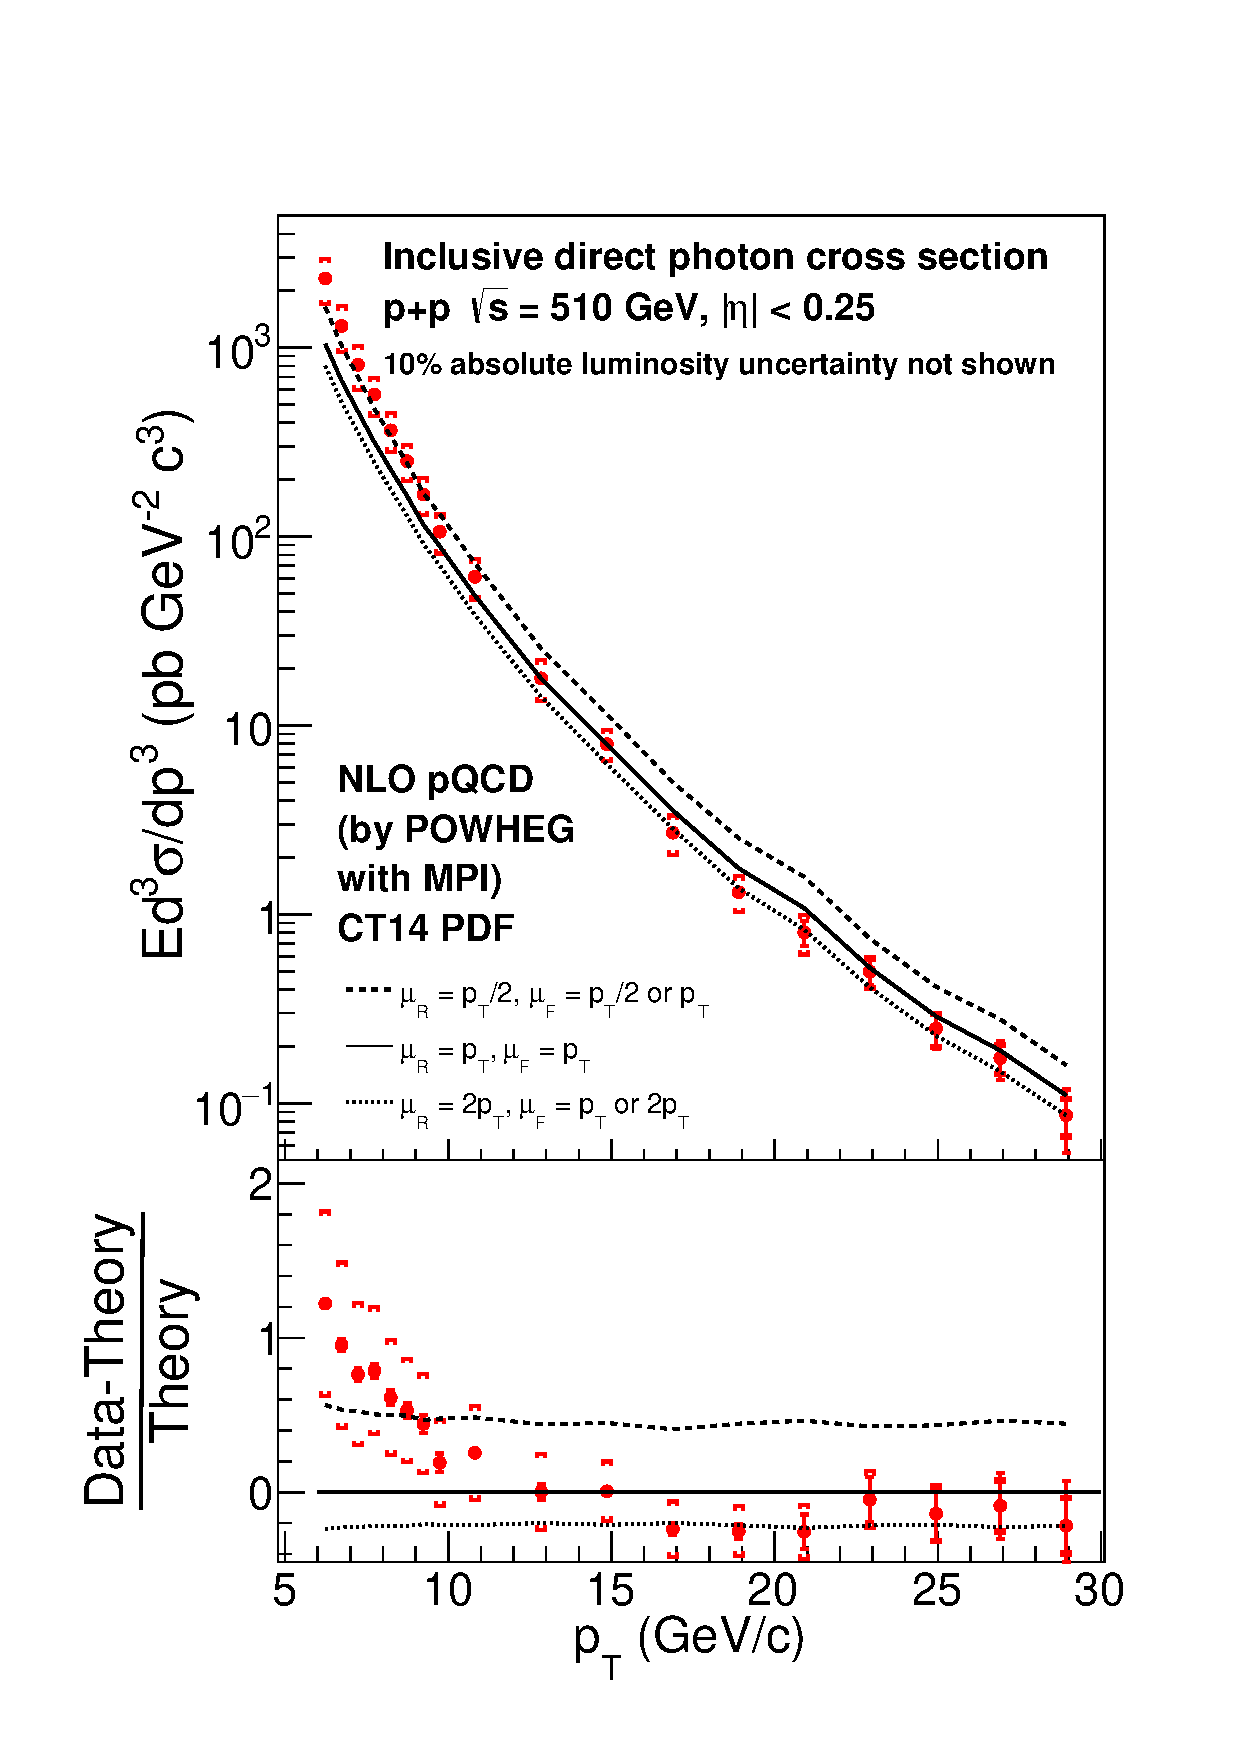
\includegraphics[width=0.5\textwidth]{CrossSection-photon-pwhg}
\caption{Inclusive direct photon cross section in proton collisions at $\sqrt{s}$ = 510 GeV measured at midrapidity. Vertical bars and square brackets show statistical and systematic uncertainties, respectively. The theoretical curves using POWHEG+PYTHIA8 are shown for different renormalization and factorization scales \cite{Nason_2004, Frixione_2007, Alioli2010, Jezo2016}. The bottom plot shows the comparison of data and calculations.}
\label{fig:inc}
\end{figure}

%systematic here
The main systematic uncertainty sources are from global energy scale of tuning the \pizero\ mass peak position and energy nonlinearity of the EMCal response at high \pT, which are calculated by a single \pizero\ or photon generator with fast detector simulation and were determined to be between 14\% and 19\% depending on \pT. The systematic uncertainties due to \pizero\ yield extraction and relative fractions of other hadron decays over \pizero\ are 2-12\% and 5-14\%, respectively. The loss of photons from conversions in material before the EMCal is estimated using a single photon generator + GEANT full detector simulation \cite{Brun:1994aa}. The material of the vertex tracker \cite{SONDHEIM2012993} leads to a (12.8 $\pm$ 1.9)\% probability for a photon to convert. Conversions in other materials lead to (3 $\pm$ 1)\% in PbSc and (4.5 $\pm$ 1.3)\% in PbGl for photon loss. This translates into relative uncertainties of 1-8\%. The uncertainties from EMCal detector resolution (2-8\%) and trigger (2-4.5\%) are also taken into account. Other uncertainties include geometrical acceptance, trigger efficiencies and pile-up effect and are in total less than 7\%.

The isolated direct photon cross section is shown in Fig.~\ref{fig:iso} as a function \pT and compared with the NLO pQCD calculation \cite{PhysRevD.48.3136,PhysRevD.50.1901} using NNPDF3.0 \cite{Ball2015,Bonvini2015} and GRV fragmentation functions (FF) \cite{PhysRevD.45.3986}. The calculation is in good agreement with our data within the uncertainties. Similar to the inclusive cross section result, the global energy scale and energy nonlinearity are the major contributions to the systematic uncertainties, which are 7-13\% depending on \pT. The systematic uncertainties due to \pizero\ yield extraction and other hadrons' production ratio are 0.5-2.5\% and 0.4-6\%, respectively. These contributions are relatively smaller than the inclusive case as the isolation requirement largely reduces these backgrounds.

\begin{figure} 
\centering
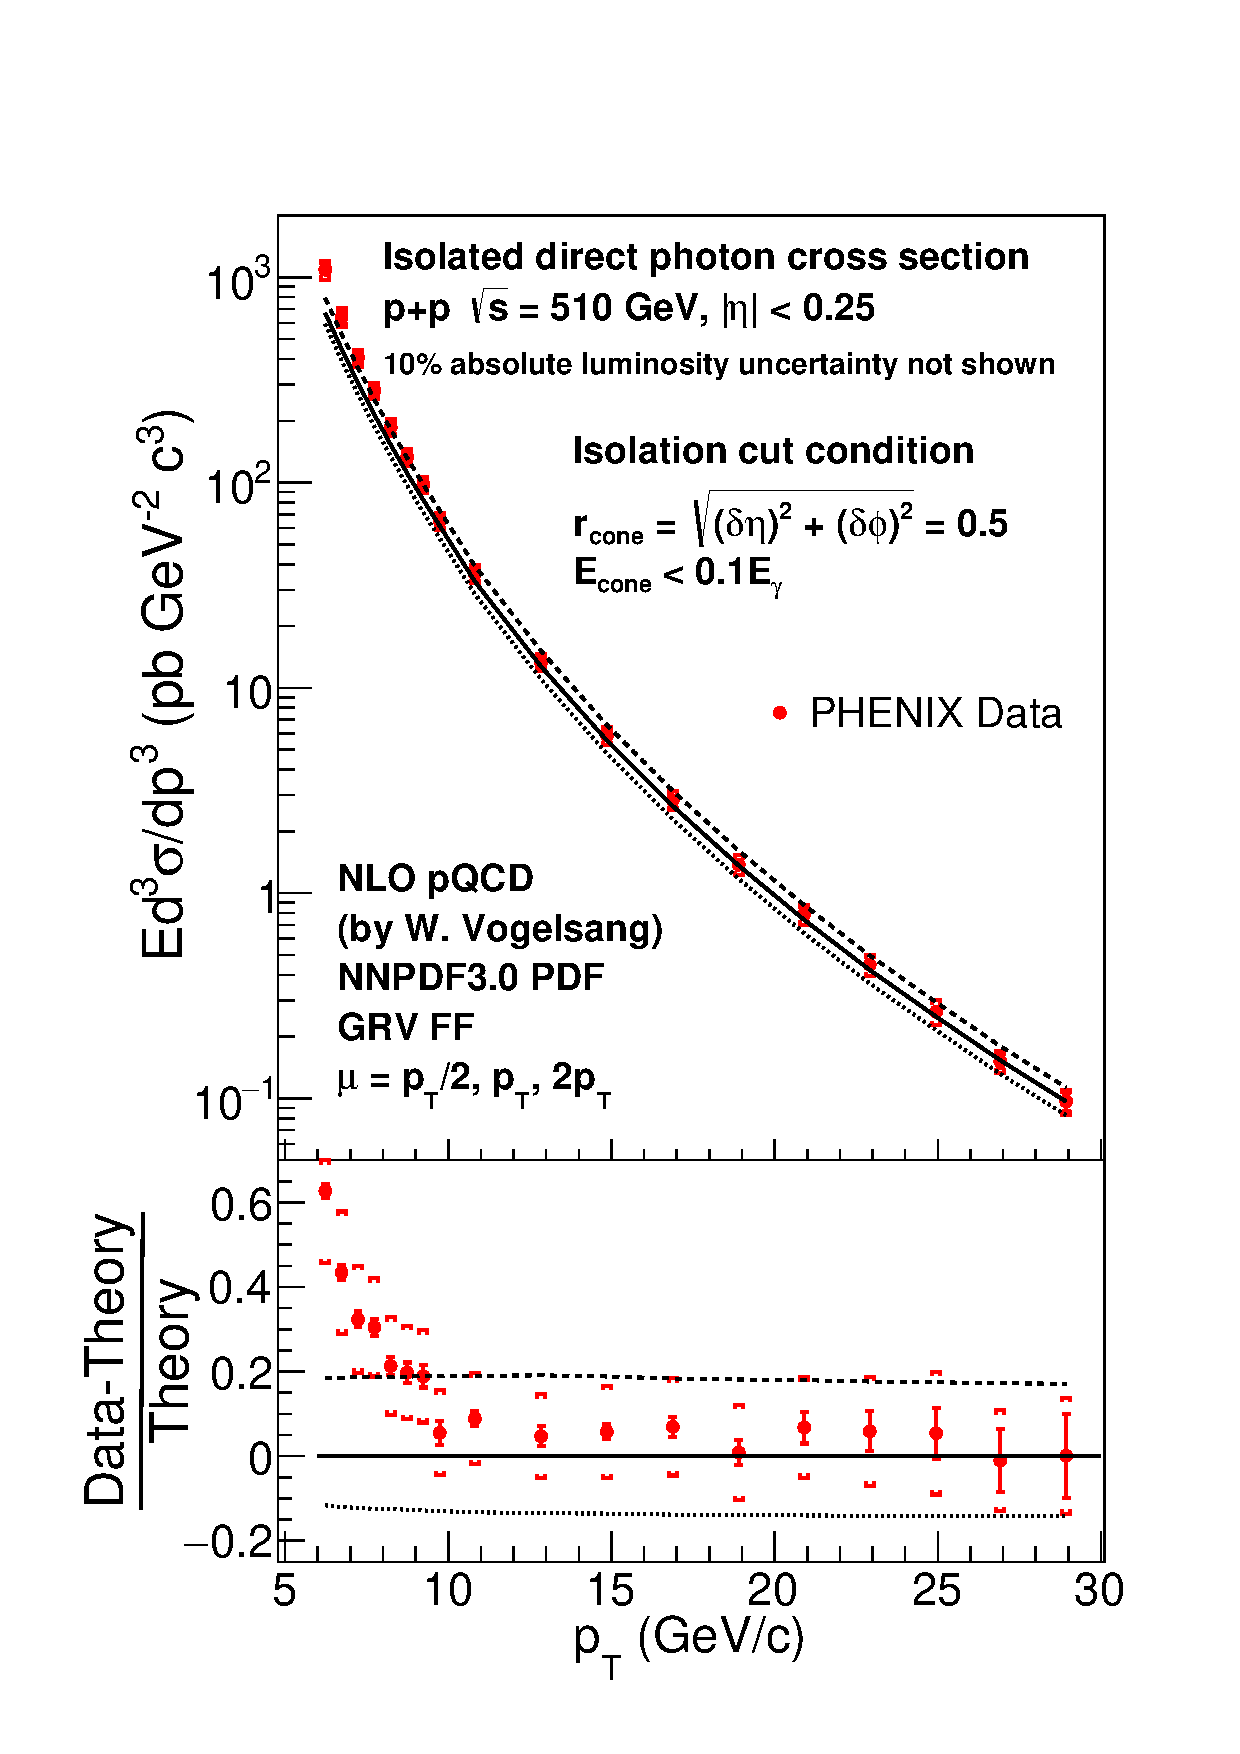
\includegraphics[width=0.5\textwidth]{CrossSection-isophoton-werner}
\caption{Isolated direct photon cross section as a function of \pT compared with NLO pQCD calculations \cite{PhysRevD.48.3136,PhysRevD.50.1901} for different renormalization and factorization scales $\mu$ = \pT/2 (dashed line), \pT (solid line), 2\pT (dotted line). The bars represent statistical uncertainties and square brackets are for systematic uncertainties. The bottom plot shows the comparison of data and calculations.}
\label{fig:iso}
\end{figure}

%\begin{table}
%\centering
%\caption{\label{tab:sys-err-sum}Summary of relative systematic uncertainties of inclusive and isolated direct photon cross sections.}
%\begin{tabular}{c c c}
%\hline
%\hline
%Source & $\Delta\sigma^{inc}_{sys}/\sigma^{inc}$ & $\Delta\sigma^{iso}_{sys}/\sigma^{iso}$ \\
%\hline
%Global energy scale and & & \\
%geometrical misalignment and & & \\
%energy nonlinearity & 14--19\% & 7--13\% \\
%EMCal resolution & 2--8\% & 0.3--3\% \\
%\pizero\ yield extraction & 2--12\% & 0.5--2.5\% \\
%$\eta$, $\omega$ and $\eta'$ prod. ratio & 5--14\% & 0.4--6\% \\
%Geometrical acceptance & $<$0.5\% & $<$1\% \\
%Photon conversion & 1--8\% & 0.5--2.5\% \\
%ERT efficiency and normalization & 2--4.5\% & 2--4.5\% \\
%MB trigger bias & 1\% & 1\% \\
%Pile-up effect & 1\% & 2\% \\
%\hline
%\hline
%\end{tabular}
%\end{table}

In Fig.~\ref{fig:iso2inc}, the ratio of isolated over inclusive direct photons is shown together with theoretical calculations. The MC simulations using POWHEG+PYTHIA8 generator were produced with and without MPI. When MPI is not included it overestimates the ratio similar to the NLO pQCD calculations using NNPDF3.0 PDF and GRV FF while including MPI shows better agreement with this measurement.

\begin{figure}
\centering
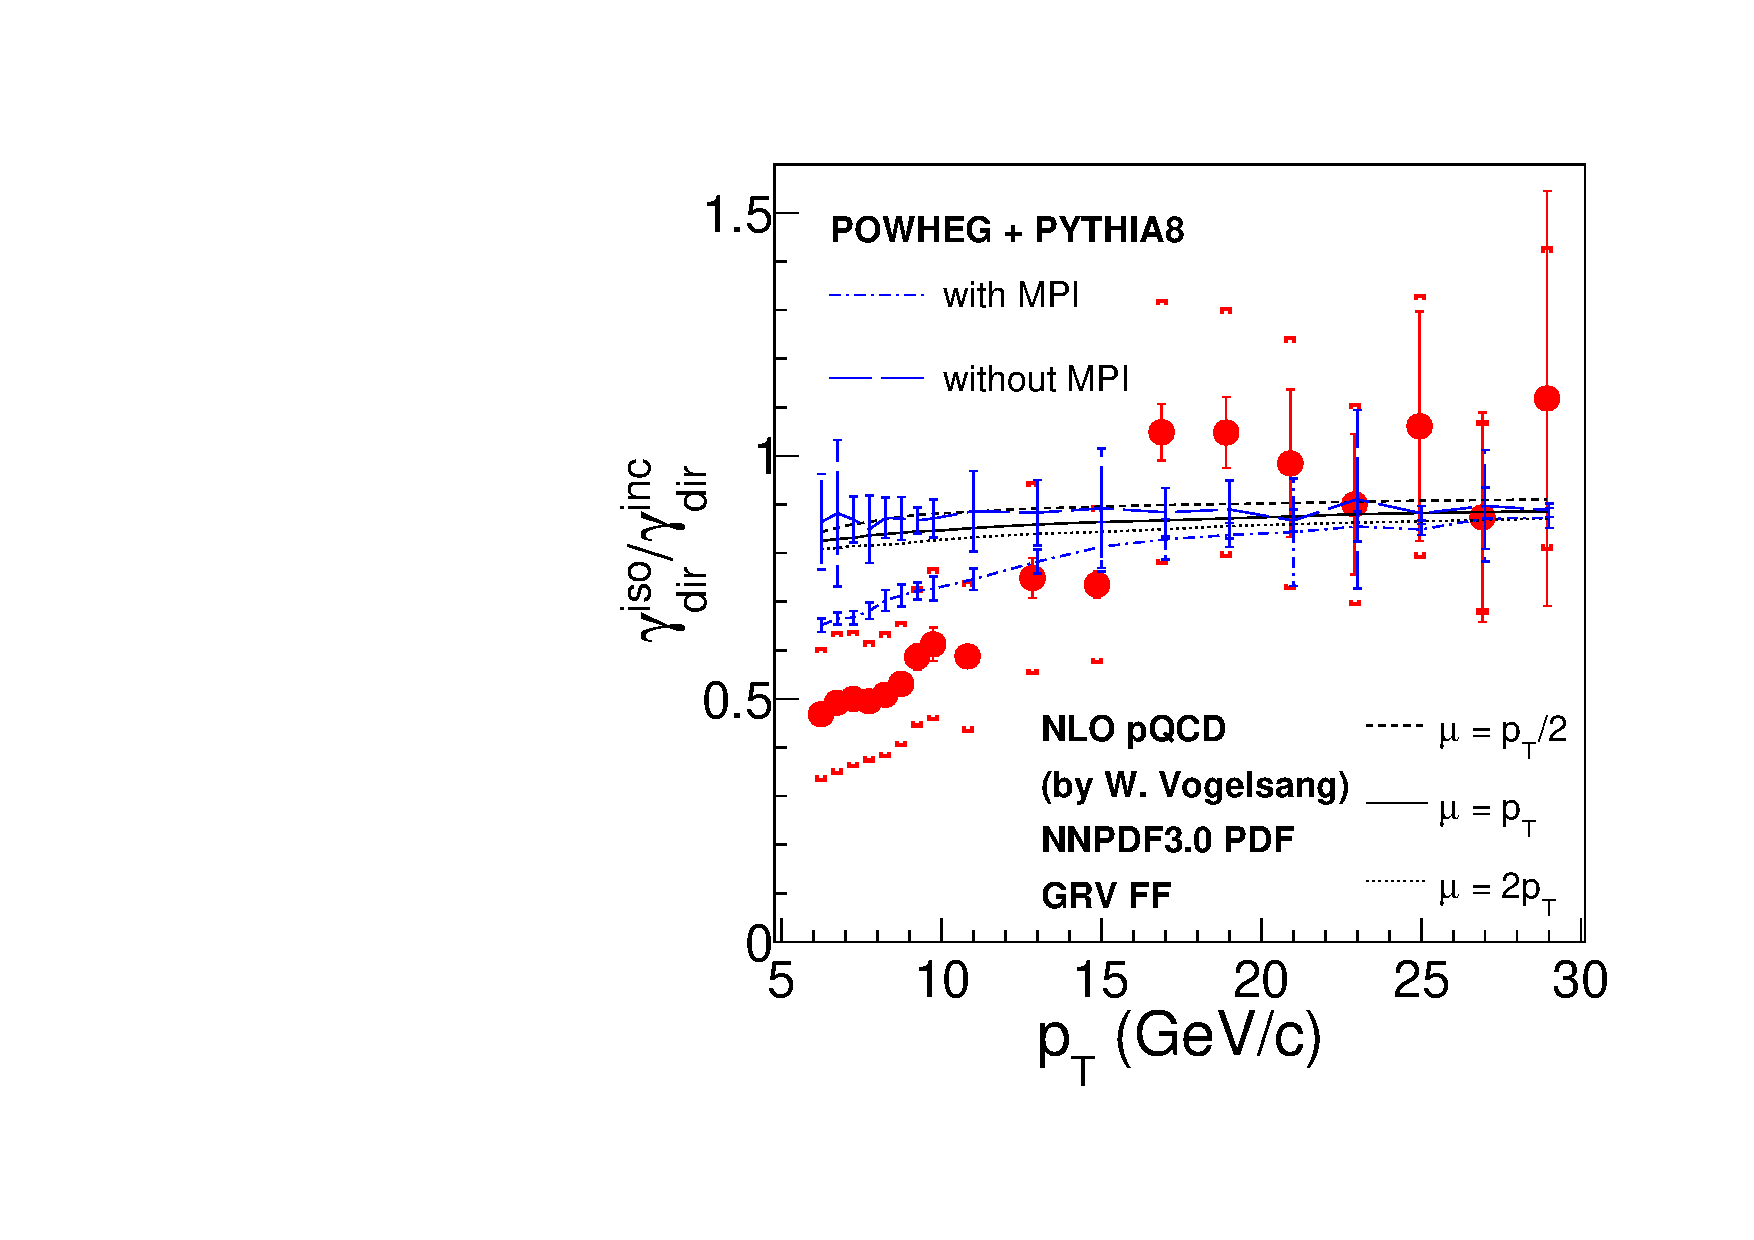
\includegraphics[width=0.5\textwidth]{Iso2Inc}
\caption{Isolated over inclusive direct photon ratio: bars are statistical uncertainties and square brackets are systematic uncertainties. POWHEG + PYTHIA8 without MPI and NLO pQCD calculations with different renormalization and factorization scales are also shown.}
\label{fig:iso2inc}
\end{figure}

The double helicity asymmetry is defined as

\begin{equation} \label{eq:all}
A_{LL} = \frac{\Delta\sigma}{\sigma} = \frac{\sigma_{++}-\sigma_{+-}}{\sigma_{++}+\sigma_{+-}},
\end{equation}
where $\sigma_{++}$ ($\sigma_{+-}$) is the cross section for the same (opposite) helicity proton collisions. This can be rewritten in terms of particle yield and beam polarizations:

\begin{equation}
A_{LL} = \frac{1}{P_BP_Y} \frac{N_{++}-RN_{+-}}{N_{++}+RN_{+-}}.
\end{equation}
where $N_{++}$ ($N_{+-}$) is the number of isolated direct photons from the bunches with the same (opposite) helicities. $P_{B}$ and $P_{Y}$ are the polarizations for the two proton beams, and the average values in 2013 were 55\% and 57\%, respectively \cite{POBLAGUEV2020164261}. $R$ $(= \mathcal{L_{++}}/\mathcal{L_{+-}}$) is the relative luminosity that is measured by the BBC. The systematic contribution of R to $A_{LL}$ was found to be 3.9 $\times$ $10^{-4}$.

The asymmetry was calculated for photon candidates that passed the same time-of-flight, minimum energy, and isolation requirements as the cross section analysis. The z-vertex requirement of 30 cm is used for the asymmetry measurement. The asymmetry contribution for background photons from \pizero's decay was calculated from the sideband region (47-97 MeV/$c^2$ and 177-227 MeV/$c^2$) around the \pizero\ mass peak (112-162 MeV/$c^2$) using the inclusive photon sample due to the limited statistics in the isolated photon sample. The asymmetry for other hadron decays (mostly $\eta$'s decay) was taken as $A_{LL}^{\eta}$ from previous PHENIX measurement at $\sqrt{s}$ = 200 GeV by assuming $x_T$ scaling (TABLE~VII of \cite{PhysRevD.90.012007}). We varied $A_{LL}^{\eta}$ by the quadratic sum of its statistical and systematic uncertainties to explore its systematic uncertainty. The background corrected asymmetry can be calculated as

\begin{equation} \label{eq:all-dir}
A_{LL}^{dir} = \frac{A_{LL}^{total} - r_{\pi^0}A_{LL}^{\pi^0} -r_h A_{LL}^{\eta}}{1 - r_{\pi^0} - r_h},
\end{equation}
where $r_{\pi^0}$ (10-14\%) and $r_h$ (0.6-1.4\%) are background fractions of \pizero\ and other hadron decay photons, respectively. Consistency checks of asymmetries were performed to ensure that there is no hidden systematic effect and the asymmetry is calculated reliably. The data were divided into subgroups according to the bunch patterns that were used to fill the RHIC rings, and calculated asymmetries were found to be consistent.

%We measure the isolated total photon $A_{LL}^{total}$ and background photons from \pizero's decay $A_{LL}^{\pi^0}$ in a run-by-run basis separated for eight groups (four patterns with even and odd crossings) and get average for each group. Since most of the other background photons are from $\eta$'s decay and $A_{LL}^{\eta}$ is consistent with zero (fig.~12 of \cite{PhysRevD.90.012007}), we use $A_{LL}^h \sim$ 0 for other hadrons' decay photons. We use the same time-of-flight requirement $|ToF| <$ 10 ns and minimum energy requirement $E_{min} >$ 0.3 GeV for the clusters. Each run must have statistics $N_{++} + N_{+-} \geq 10$. Here we use a BBC vertex requirement of $\pm$30 cm (instead of $\pm$10 cm used in cross section analysis) and a logical OR of EMCal triggers with 3.7, 4.7 or 5.6 GeV threshold. After checking consistency of the eight groups, we combine them to get the final \ALL. The isolated direct photon $A_{LL}^{dir}$ is calculated as

\begin{figure}[htb]
\centering
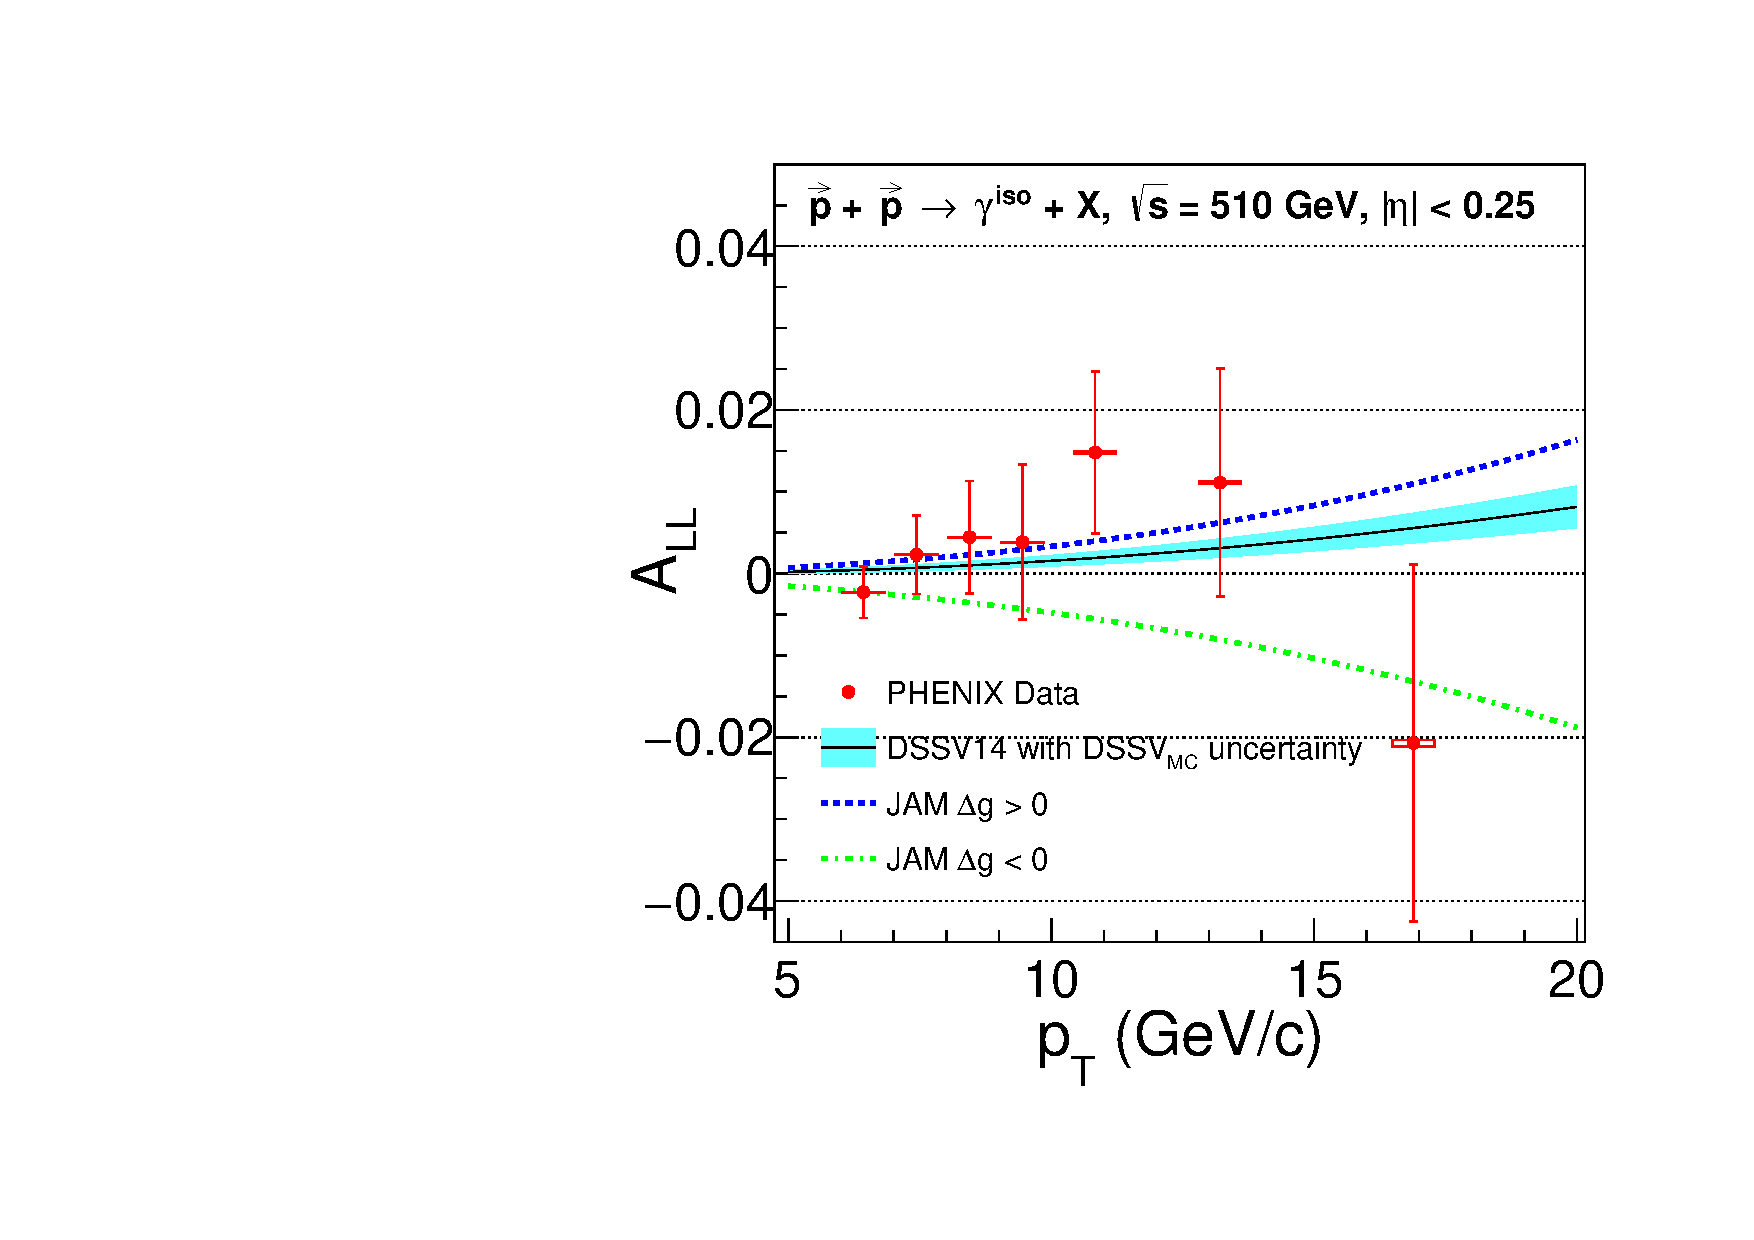
\includegraphics[width=0.5\textwidth]{IsoPhotonALL-beam2}
\caption{Double helicity asymmetry $A_{LL}$ $vs$ $p_{T}$ for isolated direct photon production in polarized p+p collisions at $\sqrt{s}$ = 510 GeV at midrapidity. Vertical error bars (boxes) represent the staistical (systematic) uncertainties. The NLO pQCD calculation is plotted as the solid curve with $1\sigma$ uncertainty band from MC replica \cite{PhysRevLett.101.072001,PhysRevLett.113.012001,PhysRevD.100.114027}.}
\label{fig:all}
\end{figure}

The double helicity asymmetry of isolated direct photon production in longitudinally polarized proton collisions at $\sqrt{s}$ = 510 GeV is shown in Fig.~\ref{fig:all} for 6 $< p_{T} <$ 20 GeV/c. The NLO pQCD calculation was obtained using DSSV14 polarized PDF, NNPDF3.0 unpolarized PDF and GRV FF for the renormalization and factorization scales $\mu = p_T$ with $1\sigma$ uncertainty band from MC replicas \cite{PhysRevLett.101.072001,PhysRevLett.113.012001,PhysRevD.100.114027}. The calculation is in good agreement with our results within the experimental uncertainties. In the asymmetry measurement systematic effects are largely canceled. The systematic uncertainties in fig.~\ref{fig:all} include point-to-point uncertainties from background estimation and false asymmetry in background due to pile-up effect at low \pT.

%\textcolor{red}{The systematic uncertainties of $A_{LL}^{dir}$ include false asymmetry in background due to pile-up effect at low \pT, $3.9\times 10^{-4}$ relative luminosity difference measured by BBC and zero degree calorimeter (ZDC) \cite{ADLER2001488}, 6.6\% global scaling uncertainty from beam polarization $P_B P_Y$, yield extraction for \pizero\ background and $A_{LL}^{\eta}$ from $\eta$ background.}

In summary, PHENIX has measured the first inclusive and isolated direct photon cross sections at midrapidity in proton collisions at $\sqrt{s}$ = 510 GeV. The NLO pQCD calculations are overall consistent with our results except at lower \pT\ where the calculations underestimate the cross sections. The calculations including underlying events such as MPI and PS give a better description for the inclusive cross section which indicates the importance of considering such contributions to understand the results at low $p_{T}$. We have measured $A_{LL}$ of isolated direct photons in longitudinally polarized proton collisions at $\sqrt{s}$ = 510 GeV. This is the first time that the direct photon has been used to probe the polarized gluon distribution inside the proton. Direct photons are free from the final-state effects and therefore can provide a clean access to gluons. The result will provide an independent constraint on the gluon spin contribution to the proton spin when included in the future global analyses.
%%% For help see /phenix/WWW/p/info/dp/000/template/template4.tex

%%% To check PRL length insert these (uncommented) lines here:
\clearpage \textbf{*** page break for PRL word count $<$3.5 pages $<$7 columns ***}

%%%%%%%%%%%%%%%%%%%%%%%%%  Acknowledgements 
% for PRC or PRD only, uncomment this line:
%\section*{ACKNOWLEDGMENTS}  

%% Acknowledgments are determined by runs for which new results are
%% being released.  As with the author lists, Brant will add later
%% by using the most current acknowledgments, plus any additions
%% from relevant runs.  For example, new Run-6 releases include:
%% "a sponsored research grant from Renaissance Technologies LLC,"

%%%%%%%%%%%%%%%%%%%%%%%%%%%  References 

\bibliography{references}   % Use of BibTeX required.

\end{document}